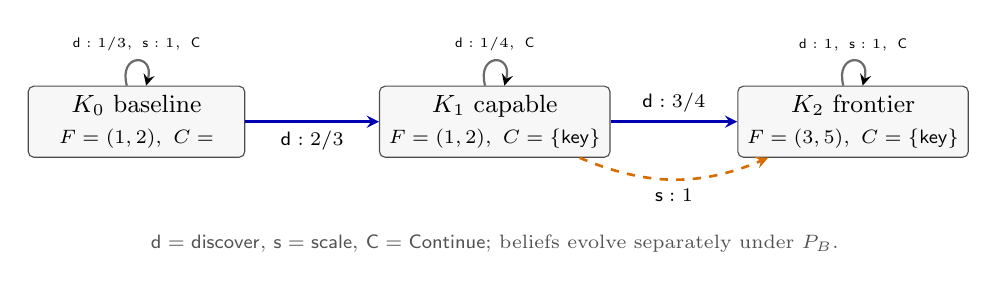
\begin{tikzpicture}[
  x=1cm,
  y=1cm,
  >=stealth,
  state/.style={
    draw=black!70,
    rounded corners=2pt,
    fill=black!3,
    minimum width=2.75cm,
    minimum height=0.88cm,
    align=center,
    font=\small
  },
  discover/.style={->,draw=blue!70!black,line width=0.95pt},
  scalearrow/.style={->,draw=orange!85!black,line width=0.95pt,dashed},
  stay/.style={->,draw=black!58,line width=0.8pt}
]
  \node[state] (k0) at (0,0)
    {\(K_0\) baseline\\{\scriptsize \(F=(1,2),\ C=\varnothing\)}};
  \node[state] (k1) at (4.55,0)
    {\(K_1\) capable\\{\scriptsize \(F=(1,2),\ C=\{\mathsf{key}\}\)}};
  \node[state] (k2) at (9.10,0)
    {\(K_2\) frontier\\{\scriptsize \(F=(3,5),\ C=\{\mathsf{key}\}\)}};

  \draw[discover] (k0) -- node[midway,below=2pt,font=\scriptsize,
    fill=white,inner sep=1pt]
    {\(\mathsf d:2/3\)} (k1);
  \draw[discover] (k1) -- node[midway,above=2pt,font=\scriptsize,
    fill=white,inner sep=1pt]
    {\(\mathsf d:3/4\)} (k2);
  \draw[scalearrow] (k1) to[bend right=23]
    node[midway,below=2pt,font=\scriptsize,fill=white,inner sep=1pt]
    {\(\mathsf s:1\)} (k2);

  \path[stay] (k0) edge[loop above,looseness=4.5]
    node[above,font=\tiny] {\(\mathsf d:1/3,\ \mathsf s:1,\ \mathsf C\)} (k0);
  \path[stay] (k1) edge[loop above,looseness=4.5]
    node[above,font=\tiny] {\(\mathsf d:1/4,\ \mathsf C\)} (k1);
  \path[stay] (k2) edge[loop above,looseness=4.5]
    node[above,font=\tiny] {\(\mathsf d:1,\ \mathsf s:1,\ \mathsf C\)} (k2);

  \node[font=\scriptsize,align=center,text=black!68] at (4.55,-1.55)
    {\(\mathsf d=\mathsf{discover}\), \(\mathsf s=\mathsf{scale}\),
     \(\mathsf C=\mathsf{Continue}\); beliefs evolve separately under \(P_B\).};
\end{tikzpicture}
